% Additional illustration 4: three weightings, one of them reported (§3.4).
% Adaptation weights over the archive define the next proposal; the
% proposal-time weight is stored with the particle and feeds parent selection
% and the online ESS; the retroactive weights over the whole history are the
% only ones that reach the reported posterior.
\documentclass[tikz,border=4pt]{standalone}
\usepackage{newtxtext,newtxmath}
\usepackage{amsmath}
\usetikzlibrary{arrows.meta,positioning,calc,fit}
\definecolor{async}{HTML}{0072B2}
\definecolor{sync}{HTML}{D55E00}
\definecolor{reject}{HTML}{009E73}

\begin{document}
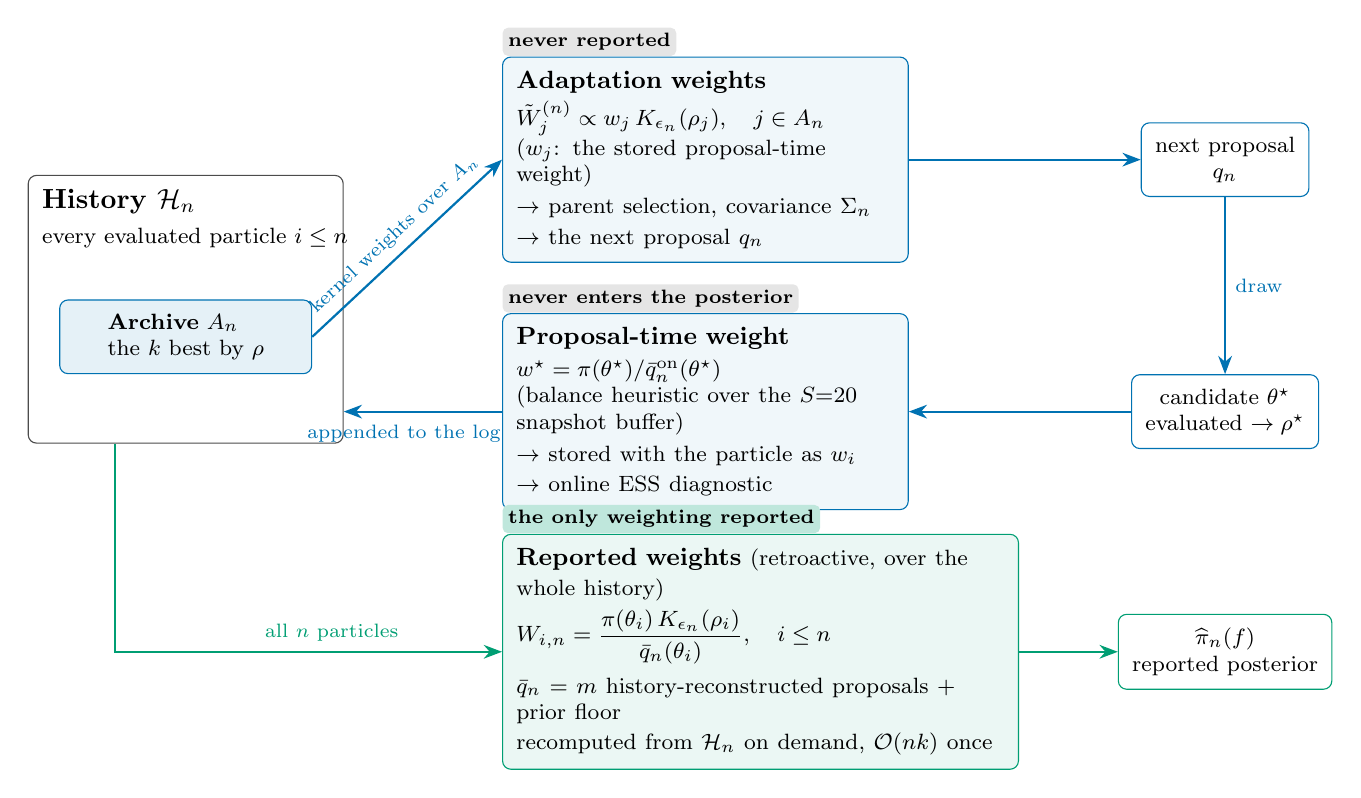
\begin{tikzpicture}[font=\small,>=Stealth,
  box/.style={draw,rounded corners=3pt,inner sep=5pt,align=left},
  tag/.style={font=\scriptsize\bfseries,inner sep=2pt,rounded corners=2pt},
  lab/.style={font=\scriptsize,text=black!70,align=center}]

%% history with the archive inside
\node[box,draw=black!70,fill=white,minimum width=4.0cm,minimum height=3.4cm] (hist) at (0,0) {};
\node[anchor=north west,font=\bfseries,inner sep=5pt] at (hist.north west) {History $\mathcal H_n$};
\node[anchor=north west,font=\footnotesize,inner sep=5pt,yshift=-14pt] at (hist.north west) {every evaluated particle $i\le n$};
\node[box,draw=async,fill=async!10,minimum width=3.2cm,align=left,font=\footnotesize] (arch) at (0,-0.35)
  {\textbf{Archive} $A_n$\\ the $k$ best by $\rho$};

%% (1) adaptation weights
\node[box,draw=async,fill=async!6,text width=4.8cm] (adapt) at (6.6,1.9) {%
  \textbf{Adaptation weights}\\[2pt]
  \footnotesize $\tilde W^{(n)}_j\propto w_j\,K_{\epsilon_n}(\rho_j),\quad j\in A_n$\\
  \footnotesize ($w_j$: the stored proposal-time weight)\\[2pt]
  \footnotesize $\to$ parent selection, covariance $\Sigma_n$\\
  \footnotesize $\to$ the next proposal $q_n$};
\node[tag,fill=black!10,anchor=south west] at (adapt.north west) {never reported};

%% (2) proposal-time weight
\node[box,draw=async,fill=async!6,text width=4.8cm] (ptw) at (6.6,-1.3) {%
  \textbf{Proposal-time weight}\\[2pt]
  \footnotesize $w^\star=\pi(\theta^\star)/\bar q^{\mathrm{on}}_n(\theta^\star)$\\
  \footnotesize (balance heuristic over the $S{=}20$ snapshot buffer)\\[2pt]
  \footnotesize $\to$ stored with the particle as $w_i$\\
  \footnotesize $\to$ online ESS diagnostic};
\node[tag,fill=black!10,anchor=south west] at (ptw.north west) {never enters the posterior};

%% (3) reported weights
\node[box,draw=reject,fill=reject!8,text width=6.2cm] (repw) at (7.3,-4.35) {%
  \textbf{Reported weights} {\footnotesize (retroactive, over the whole history)}\\[2pt]
  \footnotesize $W_{i,n}=\dfrac{\pi(\theta_i)\,K_{\epsilon_n}(\rho_i)}{\bar q_n(\theta_i)},\quad i\le n$\\[4pt]
  \footnotesize $\bar q_n$ = $m$ history-reconstructed proposals + prior floor\\
  \footnotesize recomputed from $\mathcal H_n$ on demand, $\mathcal O(nk)$ once};
\node[tag,fill=reject!25,anchor=south west] at (repw.north west) {the only weighting reported};
\node[box,draw=reject,fill=white,font=\footnotesize,align=center] (post) at (13.2,-4.35) {$\widehat\pi_n(f)$\\ reported posterior};

%% next proposal and the drawn candidate
\node[box,draw=async,fill=white,font=\footnotesize,align=center] (qn) at (13.2,1.9) {next proposal\\ $q_n$};
\node[box,draw=async,fill=white,font=\footnotesize,align=center] (cand) at (13.2,-1.3) {candidate $\theta^\star$\\ evaluated $\to\rho^\star$};

%% arrows
\draw[->,async,thick] (arch.east) -- (adapt.west) node[midway,above,sloped,lab,text=async] {kernel weights over $A_n$};
\draw[->,async,thick] (adapt.east) -- (qn.west);
\draw[->,async,thick] (qn.south) -- (cand.north) node[midway,right,lab,text=async] {draw};
\draw[->,async,thick] (cand.west) -- (ptw.east);
\draw[->,async,thick] (ptw.west) -- ($(hist.east)+(0,-1.3)$) node[pos=0.62,below,lab,text=async,yshift=-1pt] {appended to the log};
\draw[->,reject,thick] ($(hist.south)+(-0.9,0)$) |- (repw.west) node[pos=0.78,above,lab,text=reject] {all $n$ particles};
\draw[->,reject,thick] (repw.east) -- (post.west);
\end{tikzpicture}
\end{document}
